\scanpage{334}

Plus gén., si $A\supset J$ est un anneau à pd., on a $F(J)\longrightarrow F(A)$ inj., donc $F(J)$ à p. div. dans $F(A)$ ?

\diagram{\begin{tikzcd}
F(J)\arrow[r,"\mathrm{deg}\ p"] & F(J) \\
J\arrow[r,"\gamma^p",no head] & J
\end{tikzcd}}
\margin{oui, en \unsure{transf.|transportant}}

\deleted{\unsure{F}}\unsure{Je trouve la relation|Je donne la relation}
\deleted{$(x+y)$}
\[
x,y\in F(J)\quad\Longrightarrow\quad
(x+y)^{(p)}\overset{!}{=}\sum_{i+j=p}x^{(i)}y^{(j)}\quad?
\]
\[x,y\in\qquad\Vert\qquad u\]

\diagram{\begin{tikzcd}
\mathcal P\arrow[r,"\overline F",no head] & \mathcal P'
\end{tikzcd}}
commute aux produits\par
conserve degré et degrés partiels
\margin{bidegrés $1,1$}

\deleted{donc il}
\[
A,J\qquad J\longrightarrow A
\]
$A$ \deleted{ab. groupe} \inserted{$k$-} ass comm avec $1$\par
$J$ anneau ass comm sans $1$\par
$A$ opère sur $J$, et $(\lambda xy=x(\lambda y)=\lambda xy$
\[
J\xrightarrow{i} A\qquad\text{hom de }A\text{-}\text{algèbre}
\]
\[
(i(xy)=i(x)i(y)\qquad i(\lambda x)=\lambda i(x))
\]
\margin{\diagram{\begin{tikzcd}
A\times A\arrow[r] & A \\
A\times J\arrow[r] & J
\end{tikzcd}}}
\[
k\longrightarrow\operatorname{Hom}_{\mathcal P}(0,A)\qquad\text{hom d'anneaux}
\]
\deleted{\unsure{propre}}
\figure{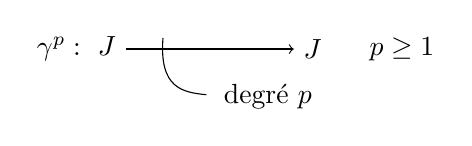
\begin{tikzpicture}
\node (source) at (0,0) {$\gamma^p:\ J$};
\node (target) at (3,0) {$J$};
\draw[->] (source.east)--(target.west);
\node[anchor=west] at (3.6,0) {$p\geq1$};
\draw (1.1,.14) .. controls (1.05,-.5) and (1.35,-.55) .. (1.65,-.58);
\node[anchor=west] at (1.75,-.6) {degré $p$};
\end{tikzpicture}}
\margin{$\gamma^0:J-A$}
\[
\begin{aligned}
\gamma^0&=1\\
\gamma^1&=\mathrm{id}_J\\
\gamma^p(x+y)&=\sum_{i+j=p}\gamma^i x\,\gamma^j y\\
\gamma^p(\lambda x)&=\lambda^p\gamma^p(x)\\
\gamma^p(x)\gamma^q(x)&=C_{pq}\gamma^{p+q}(x)\\
\gamma^p(\gamma^q(x))&=\frac{(pq)!}{(p!)^q q!}\gamma^{pq}(x)
\end{aligned}
\]

\uline{transformé en Ann}
\diagram{\begin{tikzcd}
\Gamma^*F(X)\arrow[r] & F\Gamma^*(X)
\end{tikzcd}}

\mspage{335}
